\section{附录：\trMorseHomology{}就是\trCellularHomology}
\label{sec:cellular-homology}

在这个附录中，我们将证明：一个\trMorseFunction{}与一个\trPseudogradient{}场使我们得以在\trManifold{}上定义一个\textbf{\trCellularDecomposition}（cellular decomposition），并且\trMorseComplex{}与\trCellular\trComplex{}是\trIsomorphic{}的。

我们先来回忆\trCellularDecomposition{}与\trCellular\trComplex{}的定义。随后，我们仿照 Latour~[46] 来描述与\trMorse--\trSmale{}对相联系的那个\trCellularDecomposition。\footnote{至于另一种观点，可参见 [12] 中 \trLaudenbach{}的附录。}

\subsection{\trComplex{}与\trCellularHomology}
\label{subsec:complexes-cellular-homology}

在本小节中，我们沿用 Dold 的书 [25]。一个空间 $V$ 的一个\trCellularDecomposition（这里的 $V$ 可以是任意一个分离的\trTopology{}空间；我们将把它应用到\trCompact{}\trManifold{}上）是指 $V$ 的一个由子空间组成的族 $\mathcal{E}$，它满足下列性质：
\begin{itemize}
\item $\mathcal{E}$ 的每个元素 $e$ 都\trHomeomorphic{}于一个\trOpen{}\trDisk{}；
\item $\mathcal{E}$ 构成 $V$ 的一个\trCovering{}（由互不相交的子集组成）。
\end{itemize}
这些 $e$ 称为\trCellular。$V$ 的那些维数至多为 $k$ 的\trCellular{}之并，称为 $V$ 的 $k$ 维\textbf{\trSkeleton}（skeleton），并记作 $V^{(k)}$。
\begin{itemize}
\item 对于 $\mathcal{E}$ 中每个维数为 $k$ 的 $e$，都存在一个连续映射
\[
\varPhi_e\colon\bigl(B^k,S^{k-1}\bigr)\longrightarrow\bigl(V^{(k-1)}\cup e,\;V^{(k-1)}\bigr)
\]
（称为一个\textbf{\trAttachingMap}（attachment map）），它在 $B^k-S^{k-1}$ 上的限制是到 $e$ 上的一个\trHomeomorphism。
\end{itemize}
我们将假定\trCellular{}只有有限多个。

\begin{example}\label{thm:cellular-decomposition-examples}
\begin{enumerate}[label=(\arabic*)]
\item 在维数为 $n$ 的\trSphere{}上，取一个点（比如说南极 $S$，以便说明想法）的补集，便得到一个维数为 $n$ 的\trOpen{}\trDisk{}。它与那个缺失的点一起，构成\trSphere{}的一个\trCellularDecomposition，其维数至多为 $n-1$ 的诸\trSkeleton{}全都是点 $S$。
\item \trProjectiveSpace{}是一个仿射空间与一个位于无穷远处的超平面之并，而后者又是一个仿射空间与一个无穷远超平面之并……如此等等。因此，实（或复）\trProjectiveSpace{}容许这样一个\trCellularDecomposition：在每个维数上各有一个\trCellular（相应地，在每个偶数维数上各有一个）。
\item \trTorus{} $T^2=\RR^2/\ZZ^2$——把它看成一张各边两两等同的正方形——具有一个由下述元素组成的\trCellularDecomposition：
  \begin{itemize}
  \item 一个维数为 2 的\trCellular（即那个\trOpen{}正方形）；
  \item 两个维数为 1 的\trCellular（一个来自诸水平边，另一个来自诸竖直边）；
  \item 以及一个维数为 0 的\trCellular（来自正方形的四个顶点）。
  \end{itemize}
\end{enumerate}
\end{example}

\begin{remark}\label{thm:skeleton-quotient-bouquet}
如果我们把 $(k-1)$ 维\trSkeleton{}捏缩，也就是说，如果我们取商 $V^{(k)}/V^{(k-1)}$，那么所得结果是一个维数为 $k$ 的\textbf{\trBouquetOfSpheres}（bouquet of spheres），其中每个\trSphere{}各来自一个\trCellular（即一个 $D^k$），而我们已把这个\trCellular{}边界上的全部点都等同为一点。\footnote{译注：“束”（bouquet）是\trTopology{}学的习惯说法，指把一族空间在一个公共点处\trGluing{}起来所得的空间；“由零个\trSphere{}组成的束”不外是单独一个点。}
这个束也可以是由零个\trSphere{}组成的束——维数为 $n$ 的\trSphere{}在 $k\le n-1$ 时便是这种情形。
在上文那个维数为 2 的\trTorus{}的例子里，$V^{(1)}/V^{(0)}$ 是由两个\trCircle{}组成的一个束。
\end{remark}

\trCellular\trComplex{} $K_\star$ 定义如下：取 $K_m$ 为 $\ZZ/2$ 上由维数为 $m$ 的诸\trCellular{}所生成的\trVectorSpace（或者，如果我们想定义整系数\trHomology，就取由维数为 $m$ 的诸\trCellular{}所生成的\trAbelianGroup）。

其\trDifferential{}定义为
\[
\partial c=\sum_d N(c,d)\,d\text{，}
\]
其中，与维数为 $m$ 的\trCellular{} $c$ 以及维数为 $m-1$ 的\trCellular{} $d$ 相联系的数 $N(c,d)$ 定义如下：
\begin{itemize}
\item 根据定义，\trCellular{} $c$ 是某个映射 $\varPhi_c$ 的像。
\item 我们考虑分解
\[
\varPhi_c\big|_{S^{m-1}}\colon S^{m-1}\longrightarrow V^{(m-1)}\longrightarrow V^{(m-1)}/V^{(m-2)}\text{。}
\]
\item 最后这个空间是一束 $(m-1)$ 维的\trSphere，其中有一个\trSphere{}对应于\trCellular{} $d$（正如\cref{thm:skeleton-quotient-bouquet}所指出的那样）；因此存在一个映射
\[
\varPsi_d\colon V^{(m-1)}/V^{(m-2)}\longrightarrow S^{m-1}
\]
它把除对应于 $d$ 的那个\trSphere{}之外的所有\trSphere{}都捏缩成一点。
\item 数 $N(c,d)$ 就是复合映射
\[
\varPsi_d\circ\varPhi_c\colon S^{m-1}\longrightarrow S^{m-1}
\]
的\trMappingDegree（我们模 2 地考虑它）。
\end{itemize}

可以证明（参见 [25]）：$(K_\star,\partial)$ 是一个\trComplex（$\partial\circ\partial=0$），而且这个\trComplex{}的\trHomology{}不依赖于所取的\trCellularDecomposition。

在“\trMorse--\trSmale”的语境下——也就是说，给定\trManifold{} $V$ 上的一个\trMorseFunction{}与一个\trPseudogradient{}场——我们将要构造 $V$ 的一个\trCellularDecomposition，其诸\trCellular{}将是该函数诸\trCriticalPoint{}的诸\trUnstableManifold。我们将证明下述定理。

\begin{theorem}\label{thm:morse-cellular-isomorphism}
设 $(f,X)$ 是\trManifold{} $V$ 上的一个\trMorse--\trSmale{}对。那么存在该\trManifold{}的一个\trCellularDecomposition，以及一个从\trCellular\trComplex{}到\trMorseComplex{}的\trIsomorphism
\[
F:K_\star\longrightarrow C_\star\qquad\text{满足}\qquad \partial_X\circ F=F\circ\partial\text{。}
\]
\end{theorem}

于是，\trManifold{} $V$ 的\trMorseHomology{}\trIsomorphic{}于它的\trCellularHomology{}。

如果我们在每个\trCellular{}上取定一个\trOrientation，并把 $N(c,d)\in\ZZ$ 定义为 $\varPsi_d\circ\varPhi_c$ 的\trMappingDegree，那么便得到 $\ZZ$ 上的一个\trComplex，而\cref{thm:morse-cellular-isomorphism}依然成立。

\subsection{与一个\trMorse--\trSmale{}对相联系的\trCellularDecomposition}
\label{subsec:cellular-decomposition-morse-smale}

在本小节中，我们沿用 [46] 中 Latour 的定义与想法。\trCompact{}\trManifold{} $V$ 上被赋予了一个\trMorseFunction{} $f$ 与一个\trPseudogradient{}场 $X$。我们假定 $X$ 满足\trSmale{}性质。

正如\cref{thm:stable-unstable-submanifolds}所说，$f$ 的\trCriticalPoint{}的\trUnstableManifold{}是一个开球，其维数即该\trCriticalPoint{}的\trIndex。我们首先要把这些\trUnstableManifold{}\trCompactification{}成闭球。

设 $c$ 是一个\trCriticalPoint。我们令
\[
\overline{W}^{\,u}(c)=W^u(c)\sqcup\bigcup_d\Bigl(\overline{\mathcal{L}}(c,d)\times W^u(d)\Bigr)\text{。}
\]
这个并取遍所有使得 $\overline{\mathcal{L}}(c,d)$ 非空的\trCriticalPoint{} $d$，也就是说，取遍所有与 $c$ 相连接的\trCriticalPoint。\footnote{译注：原书此式印作 $\overline{W}^{\,u}(c)=W^u(c)\cup\bigl(\overline{\mathcal{L}}(c,d)\times\bigcup_d W^u(d)\bigr)$：取并的作用域排法使第一因子 $\overline{\mathcal{L}}(c,d)$ 中的 $d$ 悬空无所指；应把 $\bigcup_d$ 置于乘积之外（且 $W^u(c)$ 由 $V$ 中的点组成、乘积块由（破碎\trTrajectory{}，点）对组成，二者互不重叠，故取\trDisjointUnion）；此处径改。——译者注}由\trSmale{}性质可知，这些点的\trIndex{}都小于 $c$ 的\trIndex。

我们现在赋予 $\overline{W}^{\,u}(c)$ 一个\trTopology{}。我们当然采用\cref{sec:space-of-connections}中在\textbf{\trMulticonnectionSpace}（multiconnection space）$\overline{\mathcal{L}}(c,d)$ 上所定义的那个\trTopology{}。设 $(\lambda,x)\in\mathcal{L}(c,d_1)\times\cdots\times\mathcal{L}(d_{k-1},d)\times W^u(d)$。我们可以把 $(\lambda,x)$ 在 $\overline{W}^{\,u}(c)$ 中的、由开邻域组成的一个基本组 $W(\lambda,x,U^0,\mathbf{U}^-,\mathbf{U}^+)$ 描述如下：
\begin{itemize}
\item 显然，$U^0$ 是 $x$ 在 $V$ 中的一个邻域。
\item $W(\lambda,\mathbf{U}^-,\mathbf{U}^+)$ 是 $\lambda$ 在 $\overline{\mathcal{L}}(c,d)$ 中的一个邻域。
\item 如果 $(\mu,x')\in\overline{\mathcal{L}}(c,d_i)\times W^u(d_i)$（对某个 $i\le k$），那么我们说\footnote{译注：原书此处印作 $W(x,\lambda,U^0,\mathbf{U}^-,\mathbf{U}^+)$；与上文定义处的 $W(\lambda,x,\dotsc)$ 实参顺序不一，系显见记号笔误；此处径依定义处统一。——译者注}
\[
(\mu,x')\in W(\lambda,x,U^0,\mathbf{U}^-,\mathbf{U}^+)\text{，}
\]
如果：
  \begin{itemize}
  \item $x'\in U^0$；
  \item 从 $d_i$ 到 $x'$ 的那条\trTrajectory{}对 $j\ge i$ 通过 $U_j^-$，而对 $j>i$ 通过 $U_j^+$；
  \item $\mu\in W(\lambda',\mathbf{U}^{-\prime},\mathbf{U}^{+\prime})$（其中 $\lambda'=(\lambda_1,\dotsc,\lambda_i)$，而诸 $\mathbf{U}^{\pm\prime}$ 的定义则一如你所想）。
  \end{itemize}
\end{itemize}

例如，如果 $c$ 是一个\trIndex{}为 0 的\trCriticalPoint，那么 $W^u(c)=\{c\}$，$\overline{W}^{\,u}(c)$ 亦然（这确实是一个维数为 0 的\trCellular）。下面来看一些不那么平凡的例子。

\begin{example}\label{thm:closed-cell-examples}
\begin{enumerate}[label=(\arabic*)]
\item 设 $c$ 是一个\trIndex{}为 1 的\trCriticalPoint。那么 $W^u(c)$ 由 $V$ 上位于那些从 $c$ 通到\trIndex{}为 0 的\trCriticalPoint{}的\trTrajectory{}之上的点组成——这样的\trTrajectory{}有两条，它们在 $V$ 中的端点便是这两个（或者这同一个）\trCriticalPoint。在 $\overline{W}^{\,u}(c)$ 中，我们为每一条这样的\trTrajectory{}都添上一个点。无论它们的端点是否相同，这两条\trTrajectory{}都给出相异的两个点：$\mathcal{L}(c,d)\times W^u(d)$ 含有点 $\{\ell_1\}\times\{d\}$ 与 $\{\ell_2\}\times\{d\}$。于是 $\overline{W}^{\,u}(c)$ 是一个维数为 1 的\trClosed{}\trDisk{}（\cref{fig:index-one-critical}）。

\setcounter{figure}{6}%
\begin{figure}[htbp]
\centering
\begin{tikzpicture}[line width=0.6pt,scale=0.9]
  \begin{scope}
    \draw plot[domain=-2.3:2.3] (\x,{0.30*\x*\x+0.85});
    \draw plot[domain=-2.3:2.3] (\x,{0.30*\x*\x-0.85});
    \draw (0,0.85) arc (90:-90:0.55 and 0.85);
    \draw[dashed] (0,0.85) arc (90:270:0.55 and 0.85);
    \draw[dashed,->] (-0.537,0.176) arc (168:192:0.55 and 0.85);
    \draw[->] (0.537,0.176) arc (12:-12:0.55 and 0.85);
    \fill (0,0.85) circle (1.6pt);
    \fill (0,-0.85) circle (1.6pt);
  \end{scope}
  \begin{scope}[xshift=4.6cm]
    \draw (3.0,0.05) arc (180:0:0.8 and 1.15);
    \fill (3.8,1.2) circle (1.6pt);
    \draw[->] (3.13,0.68) -- (3.05,0.38);
    \draw[->] (4.47,0.68) -- (4.55,0.38);
    \draw (5.1,0.05) arc (180:0:0.8 and 1.15);
    \fill (5.9,1.2) circle (1.6pt);
    \fill (5.1,0.05) circle (1.6pt);
    \fill (6.7,0.05) circle (1.6pt);
  \end{scope}
\end{tikzpicture}
\caption{\trIndex{}为~1 的\trCriticalPoint}
\label{fig:index-one-critical}
\end{figure}

\item 其次，设 $c$ 是一个\trIndex{}为 2 的\trCriticalPoint{}。它的\trUnstableManifold{}是一个维数为 2 的\trOpen{}\trDisk{}。我们来看看需要在它上面添加些什么：
\begin{itemize}
\item 对每个与 $c$ 相连接的、\trIndex{}为 1 的\trCriticalPoint{} $d$，我们添加 $\overline{\mathcal{L}}(c,d)=\mathcal{L}(c,d)$（即从 $c$ 到 $d$ 的诸\trTrajectory，所论的每条\trTrajectory{}各对应一点）与它的\trUnstableManifold{} $W^u(d)$（一个\trOpen{}区间，如上所述）这两者的乘积。
\item 对每个与 $c$ 相连接的、\trIndex{}为 0 的\trCriticalPoint{} $e$，我们添加下述乘积：一端是从 $c$ 到 $e$ 的诸\trTrajectory{}所成之集（一些\trOpen{}线段，连同它们的边界——也就是破碎\trTrajectory{}之集，正是它把这些线段与那些连接 $c$ 及诸\trIndex{}为 1 的\trCriticalPoint{}的\trTrajectory{}联系起来），另一端是它的\trUnstableManifold（即点 $e$ 本身）。
\end{itemize}

\cref{fig:index-two-critical}在维数为 2 的情形画出了一个\trIndex{}为 2 的\trCriticalPoint{} $c$（粗点）的例子，它与唯一的\trIndex{}为 1 的\trCriticalPoint{} $d$、唯一的\trIndex{}为 0 的\trCriticalPoint{} $e$ 相连接。左图画的是这个（高度）函数的三个\trCriticalPoint，右图画的是闭“\trCellular”$\overline{W}^{\,u}(c)$，其中有：
\begin{itemize}
\item 点 $c$ 及其\trUnstableManifold{} $W^u(c)$（一个维数为 2 的\trOpen{}\trDisk）。
\item 从 $c$ 到 $d$ 的唯一\trTrajectory{} $\mathcal{L}(c,d)$，图中以小空圈表示（它象征着左图中的点 $d$）。
\item 在这个\trDisk{}的边界上我们看到乘积 $\mathcal{L}(c,d)\times W^u(d)$；由于 $\mathcal{L}(c,d)$ 仅含一个点，这个乘积就是 $d$ 的\trUnstableManifold，亦即一条\trOpen{}线段（图中以粗线段表示），它由从 $c$ 到 $d$ 的那两条\trTrajectory{}组成。\footnote{译注：原书末句作“由从 $c$ 到 $d$ 的那两条\trTrajectory{}组成”；然上文刚说 $\mathcal{L}(c,d)$ 仅含一条\trTrajectory{}（图中一个小空圈），两处自相矛盾。粗线段是 $\{\ell\}\times W^u(d)$，其成分应是 $W^u(d)$，即自 $d$ 下行通往 $e$ 的那两条分支（在闭包中连同点 $d$）；从 $c$ 到 $d$ 的\trTrajectory{}在\trCellular{}中仅以单点的身份出现（如 $\{\ell\}\times\{d\}$ 一类的极限点）。原书如此，照排。——译者注}
\item \trIndex{}为 0 的点 $e$ 的\trUnstableManifold{}当然只是一个单点。
\item 这个\trDisk{}的边界还包含 $\overline{\mathcal{L}}(c,e)\times W^u(e)$，也就是由从 $c$ 到 $e$ 的诸\trTrajectory{}所构成的那条\trOpen{}线段 $\mathcal{L}(c,e)$——图中把它画成一条圆弧——以及从 $c$ 到 $e$（途经 $d$）的那两条破碎\trTrajectory，它们正是粗线段与细圆弧的公共端点。
\end{itemize}
\end{enumerate}
\end{example}

\begin{figure}[htbp]
\centering
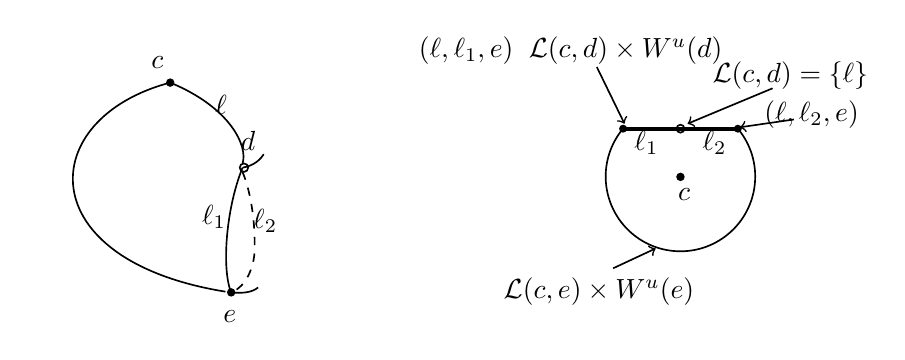
\begin{tikzpicture}[line width=0.6pt,scale=0.9]
  \begin{scope}
    \fill (0,3.0) circle (1.7pt);
    \node at (-0.18,3.28) {$c$};
    \draw (0,3.0) .. controls (-1.9,2.5) and (-2.0,0.5) .. (0.78,0.05);
    \draw (0,3.0) .. controls (0.85,2.65) and (1.1,2.1) .. (1.02,1.86);
    \draw (1.02,1.80) .. controls (1.20,1.83) and (1.28,1.93) .. (1.32,1.99);
    \draw (1.02,1.80) .. controls (0.86,1.40) and (0.80,0.95) .. (0.79,0.65)
          .. controls (0.78,0.38) and (0.81,0.15) .. (0.86,0.04);
    \draw[dashed] (1.02,1.74) .. controls (1.16,1.40) and (1.20,0.95) .. (1.19,0.62)
          .. controls (1.18,0.38) and (1.06,0.12) .. (0.88,0.05);
    \draw (0.86,0.04) .. controls (1.05,0.02) and (1.17,0.05) .. (1.24,0.11);
    \fill (0.86,0.04) circle (1.7pt);
    \draw (1.04,1.8) circle (1.7pt);
    \node at (0.72,2.68) {$\ell$};
    \node at (1.10,2.18) {$d$};
    \node at (0.62,1.10) {$\ell_1$};
    \node at (1.34,1.05) {$\ell_2$};
    \node at (0.84,-0.3) {$e$};
  \end{scope}
  \begin{scope}[xshift=4.9cm]
    \draw[line width=1.5pt] (1.49,2.35) -- (3.11,2.35);
    \draw (3.11,2.35) arc (39.8:-219.8:1.055);
    \fill (1.49,2.35) circle (1.6pt);
    \fill (3.11,2.35) circle (1.6pt);
    \draw (2.3,2.35) circle (1.6pt);
    \fill (2.3,1.67) circle (1.7pt);
    \node at (2.35,1.42) {$c$};
    \node at (1.82,2.15) {$\ell_1$};
    \node at (2.78,2.15) {$\ell_2$};
    \node at (0.75,3.45) {$(\ell,\ell_1,e)\;\;\mathcal{L}(c,d)\times W^u(d)$};
    \draw[->] (1.12,3.22) -- (1.51,2.42);
    \node at (3.85,3.10) {$\mathcal{L}(c,d)=\{\ell\}$};
    \draw[->] (3.60,2.92) -- (2.40,2.42);
    \node at (4.15,2.55) {$(\ell,\ell_2,e)$};
    \draw[->] (3.90,2.48) -- (3.14,2.37);
    \node at (1.15,0.05) {$\mathcal{L}(c,e)\times W^u(e)$};
    \draw[->] (1.35,0.38) -- (1.95,0.66);
  \end{scope}
\end{tikzpicture}
\caption{\trIndex{}为~2 的\trCriticalPoint}
\label{fig:index-two-critical}
\end{figure}

接下来我们要证明：诸 $W^u(c)$ 给出 $V$ 的一个\trCellularDecomposition，其中诸\trAttachingMap{} $\varPhi_c$ 在 $W^u(c)$ 上由包含关系给出，而在“边界”上则由它们在每一“块”上的限制给出，也就是由下述投影给出：
\[
\varPhi_c\big|_{\overline{\mathcal{L}}(c,d)\times W^u(d)}\colon
\overline{\mathcal{L}}(c,d)\times W^u(d)\longrightarrow W^u(d)\subset V\text{。}
\]

我们先来看几个例子。对于前文用过的那几个\trMorseFunction{}与\trPseudogradient{}场的例子，我们给出各种\trCellular{}的完整描述。

\begin{example}\label{thm:cell-examples-sphere-torus}
\begin{enumerate}[label=(\arabic*)]
\item 圆\trSphere。对于维数为 2 的圆\trSphere{}上的\trHeightFunction{}来说，情况十分简单。设 $a$ 为极大点、$b$ 为极小点。$a$ 附近那个维数为 2 的\trCellular{}由一个\trOpen{}\trDisk{}（即\trUnstableManifold{} $W^u(a)$）与位于边界处的\trCircle{} $\mathcal{L}(a,b)\times W^u(b)$ 组成。\trAttachingMap{}把 $\mathcal{L}(a,b)\times W^u(b)$ 捏缩到点 $W^u(b)$ 上。这样，我们便得到把该\trSphere{}分解成一个维数为 0 的\trCellular{}与一个维数为 2 的\trCellular{}的\trCellularDecomposition。
\item “另一个”\trSphere{}的例子就是\cref{fig:index-two-critical}所画的那一个。
\item \trTorus。\cref{fig:torus-index-two}的左图画出的是\trTorus{}上的\trMorseFunction{}连同\cref{subsec:examples-stable-unstable}中所给出的那个\trPseudogradient，右图画出的则是\trIndex{}为 2 的那个\trCriticalPoint{}周围的闭\trCellular。为了表示这个维数为 2 的\trCellular，我们像\cref{fig:index-two-critical}中那样，用小空圈表示诸 $\mathcal{L}(c,d_i)$，用粗线段表示诸 $\mathcal{L}(c,d_i)\times W^u(d_i)$，而用（圆）弧表示 $\mathcal{L}(c,e)\times W^u(e)$。
\end{enumerate}
\end{example}

\begin{figure}[htbp]
\centering
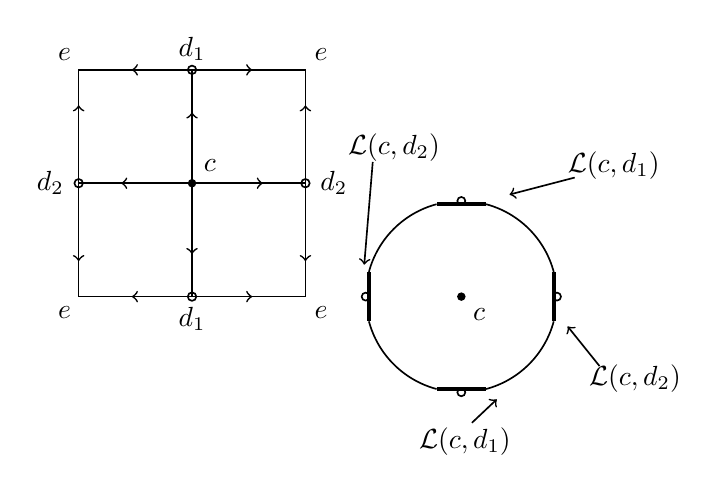
\begin{tikzpicture}[line width=0.6pt,scale=0.9]
  \begin{scope}
    \draw (0,0) rectangle (3.2,3.2);
    \draw[->] (1.35,3.2) -- (0.75,3.2);
    \draw[->] (1.85,3.2) -- (2.45,3.2);
    \draw[->] (1.35,0) -- (0.75,0);
    \draw[->] (1.85,0) -- (2.45,0);
    \draw[->] (0,2.1) -- (0,2.7);
    \draw[->] (0,1.1) -- (0,0.5);
    \draw[->] (3.2,2.1) -- (3.2,2.7);
    \draw[->] (3.2,1.1) -- (3.2,0.5);
    \draw (1.6,0) -- (1.6,3.2);
    \draw[->] (1.6,2.0) -- (1.6,2.6);
    \draw[->] (1.6,1.2) -- (1.6,0.6);
    \draw (0,1.6) -- (3.2,1.6);
    \draw[->] (1.2,1.6) -- (0.6,1.6);
    \draw[->] (2.0,1.6) -- (2.6,1.6);
    \draw (1.6,3.2) circle (1.7pt);
    \draw (1.6,0) circle (1.7pt);
    \draw (0,1.6) circle (1.7pt);
    \draw (3.2,1.6) circle (1.7pt);
    \fill (1.6,1.6) circle (1.7pt);
    \node at (-0.2,3.42) {$e$};
    \node at (3.42,3.42) {$e$};
    \node at (-0.2,-0.22) {$e$};
    \node at (3.42,-0.22) {$e$};
    \node at (1.6,3.5) {$d_1$};
    \node at (1.6,-0.32) {$d_1$};
    \node at (-0.4,1.6) {$d_2$};
    \node at (3.6,1.6) {$d_2$};
    \node at (1.85,1.85) {$c$};
  \end{scope}
  \begin{scope}[xshift=5.4cm]
    \draw[line width=1.5pt] ({1.35*cos(75)},{1.35*sin(75)}) -- ({1.35*cos(105)},{1.35*sin(105)});
    \draw[line width=1.5pt] ({1.35*cos(165)},{1.35*sin(165)}) -- ({1.35*cos(195)},{1.35*sin(195)});
    \draw[line width=1.5pt] ({1.35*cos(255)},{1.35*sin(255)}) -- ({1.35*cos(285)},{1.35*sin(285)});
    \draw[line width=1.5pt] ({1.35*cos(345)},{1.35*sin(345)}) -- ({1.35*cos(15)},{1.35*sin(15)});
    \draw ({1.35*cos(105)},{1.35*sin(105)}) arc (105:165:1.35);
    \draw ({1.35*cos(195)},{1.35*sin(195)}) arc (195:255:1.35);
    \draw ({1.35*cos(285)},{1.35*sin(285)}) arc (285:345:1.35);
    \draw ({1.35*cos(15)},{1.35*sin(15)}) arc (15:75:1.35);
    \draw (0,{1.35}) circle (1.6pt);
    \draw (0,{-1.35}) circle (1.6pt);
    \draw ({-1.35},0) circle (1.6pt);
    \draw ({1.35},0) circle (1.6pt);
    \fill (0,0) circle (1.7pt);
    \node at (0.25,-0.25) {$c$};
    \node at (2.15,1.85) {$\mathcal{L}(c,d_1)$};
    \draw[->] (1.6,1.68) -- (0.68,1.44);
    \node at (0.05,-2.05) {$\mathcal{L}(c,d_1)$};
    \draw[->] (0.15,-1.78) -- (0.5,-1.45);
    \node at (-0.95,2.1) {$\mathcal{L}(c,d_2)$};
    \draw[->] (-1.25,1.9) -- (-1.37,0.45);
    \node at (2.45,-1.15) {$\mathcal{L}(c,d_2)$};
    \draw[->] (1.95,-0.98) -- (1.5,-0.42);
  \end{scope}
\end{tikzpicture}
\caption{\trTorus{}上\trIndex{}为~2 的\trCriticalPoint}
\label{fig:torus-index-two}
\end{figure}

\subsection{定理 4.9.3 的证明}%
\label{subsec:proof-main-theorem}

我们必须证明两件事：
\begin{enumerate}[label=(\arabic*)]
\item 诸 $\overline{W}^{\,u}(c)$ 确实给出 $V$ 的一个\trCellularDecomposition；
\item 这两个\trComplex{}\trIsomorphic。
\end{enumerate}
让我们从第二个结论开始。

\textbf{\trComplex{}的\trIsomorphism}

\trComplex{} $K_\star$ 已在\cref{subsec:complexes-cellular-homology}中定义，其中每个\trCellular{}都由一个\trCriticalPoint{}的\trUnstableManifold{}给出。映射 $F$ 把这个\trCriticalPoint{}送到该\trCellular{}。\footnote{译注：定理陈述中 $F\colon K_\star\to C_\star$ 是从\trCellular\trComplex{}到\trMorseComplex{}的\trIsomorphism，本句“把\trCriticalPoint{}送到\trCellular{}”方向恰与之相反；按 $F$ 的方向宜说成“把该\trCellular{}送到（生成它的）那个\trCriticalPoint{}”，反向的陈述则应经 $F^{-1}$；此处照原书排印。——译者注}于是 $F$ 显然是\trBijective{}的。

它是\trComplex{}之间的\trIsomorphism，因为定义 $K_\star$ 的\trDifferential{}的那个数 $N(c,d)$ 就等于连接 $c$ 与 $d$ 的\trTrajectory{}的条数，也就是说，等于定义\trMorseComplex{}的\trDifferential{}的那个 $n(c,d)$。

事实上，当 $m=\operatorname{Ind}(c)$ 时，$N(c,d)$ 就是上文所定义的映射 $\varPsi_d\circ\varPhi_c:S^{m-1}\to S^{m-1}$ 的\trMappingDegree。这个映射的源是 $\overline{W}^{\,u}(c)$ 的边界——对此我们此刻暂且承认它是一个\trSphere（这是本小节所要证明的结果之一）。这个映射的靶，则是把 $(m-2)$ 维\trSkeleton{}以及那些不对应于 $d$ 的\trSphere{}统统捏缩之后所得的商，也就是 $\overline{D}^{m-1}/\partial\overline{D}^{m-1}$。我们也可以把这个商看成 $D^{m-1}$ 添加一点之后的\trCompactification，其中\trOpen{}\trDisk{} $D^{m-1}$ 被等同于\trUnstableManifold{} $W^u(d)\subset V$。如果 $\ell\in\mathcal{L}(c,d)$，那么对 $m\in W^u(d)$ 我们有
\[
\varPsi_d\circ\varPhi_c(\ell,m)=m
\]
而 $\overline{W}^{\,u}(c)$ 的边界上的其他点则被送到边界之像的那个点上去。

于是，在 $S^{m-1}$ 上我们有 $n(c,d)$ 个（即连接 $c$ 与 $d$ 的\trTrajectory{}的条数）互不相交的\trDisk，它们经\trHomeomorphism{}被送到 $D^{m-1}\subset S^{m-1}$ 上，而补集的像则是剩下的那个点。因此，\trMappingDegree{} $N(c,d)$ 确实就是\trTrajectory{}的条数 $n(c,d)$。

\textbf{\trCellularDecomposition}

我们已经见到（\cref{thm:stable-unstable-submanifolds}），\trCriticalPoint{} $c$ 的\trUnstableManifold{} $W^u(c)$ 是一个开球，其维数为 $c$ 的\trIndex。$\varPhi_c$ 在 $W^u(c)$ 上的限制是一个\trHomeomorphism，而且它的像包含在 $V^{\operatorname{Ind}(c)}$ 之中。我们必须证明：$\overline{W}^{\,u}(c)$ \trHomeomorphic{}于一个同维数的（闭）球，且其内部恰为 $W^u(c)$。

为此，对每个 $A\in\RR$，考虑
\[
\overline{W}^{\,u}(c,A)=\bigl\{(x,\lambda)\in\overline{W}^{\,u}(c)\mid f(x)\ge A\bigr\}
\]
与
\[
W^u(c,A)=\bigl\{(x,\lambda)\in W^u(c)\mid f(x)\ge A\bigr\}\text{。}
\]

当 $A=f(c)-\varepsilon$ 而 $\varepsilon$ 充分小时，
\[
\overline{W}^{\,u}(c,A)=W^u(c)\cap\overline{\Omega}(c)\text{，}
\]
其中 $\Omega(c)$ 是\trMorseChart{}中对应于参数 $\varepsilon$ 的那个\trOpen{}集，因此 $\overline{W}^{\,u}(c,A)$ 显然\trHomeomorphic{}于一个闭球。

当 $A<\min(f)$ 时，显然有
\[
\overline{W}^{\,u}(c,A)=\overline{W}^{\,u}(c)\text{。}
\]

因此我们必须证明：当 $A$ 从 $f(c)-\varepsilon$ 递减到非常负的值时，$\overline{W}^{\,u}(c,A)$ 上的\trTopology{}并不改变。下面就是一个可以轻易证明这件事的情形。

\begin{proposition}\label{thm:no-critical-interval-homeomorphism}
如果区间 $[B,A]$ 不含 $f$ 的任何\trCriticalValue，那么 $\overline{W}^{\,u}(c,A)$ 与 $\overline{W}^{\,u}(c,B)$ \trHomeomorphic。此外，这个\trHomeomorphism{}（它把 $W^u(c,A)$ 映满 $W^u(c,B)$）还可以选成在 $\overline{W}^{\,u}(c,A+\delta)$（$\delta>0$）上为恒等。\footnote{译注：原书此处插语悬空排作 “(sends $W^u(c,A)$ onto $W^u(c,B)$ and) can also be chosen equal to the identity…”，and 被置于插语末尾，致句法不整；按文义应为一个修饰\trHomeomorphic{}的插语；此处并入正文译出。——译者注}
\end{proposition}

\begin{proof}
把\cref{thm:sublevel-no-critical}应用于 $-f$ 的诸\trSublevelSet，便给出一个\trDiffeomorphism
\[
\varGamma:\{f(x)\ge A\}\longrightarrow\{f(x)\ge B\}\text{。}
\]
公式
\[
\begin{aligned}
\chi\colon\overline{W}^{\,u}(c,A)&\longrightarrow\overline{W}^{\,u}(c,B)\\
(\lambda,x)&\longmapsto(\lambda,\varGamma(x))
\end{aligned}
\]
定义了一个具备所述性质的\trHomeomorphism{} $\chi$。
\end{proof}

剩下要弄懂的，是当 $A$ 跨越一个\trCriticalValue{}时 $\overline{W}^{\,u}(c,A)$ 会发生什么。正如\cref{subsec:existence}中那样，我们假定 $f$ 的诸\trCriticalValue{}互不相同。我们有下述结果。

\begin{proposition}\label{thm:crossing-critical-value-homeomorphism}
设 $d\in\operatorname{Crit}(f)$，设 $A=f(d)$，并设 $\varepsilon>0$（它定义了一张\trMorseChart{} $\Omega(d)$）。那么存在一个\trHomeomorphism
\[
\overline{W}^{\,u}(c,A+\varepsilon)\longrightarrow\overline{W}^{\,u}(c,A-\varepsilon)
\]
（它把 $W^u(c,A+\varepsilon)$ 映满 $W^u(c,A-\varepsilon)$）\footnote{译注：这一括注附加结论照原书排印，但按其所云并不成立：$W^u(c,A+\varepsilon)$ 是闭\trDisk{}（紧），而 $W^u(c,A-\varepsilon)$ 不是——通往 $d$ 的诸\trTrajectory{}整条含于其中（$f$ 沿之始终 $\ge A-\varepsilon$、只在极限处趋于 $f(d)$），无端点可截，故 $W^u(c,A-\varepsilon)$ 非紧；紧与非紧之间不可能有映满的\trHomeomorphism。附加结论应改述为\trClosed\trCellular{} $\overline{W}^{\,u}(c,A+\varepsilon)$ 与 $\overline{W}^{\,u}(c,A-\varepsilon)$ 之间的\trHomeomorphism（即命题的主结论本身），并删去保截集的要求——证明之末重述的 $\chi\bigl(W^u(c,A+\varepsilon)\bigr)=W^u(c,A-\varepsilon)$ 同此。又，$\operatorname{Ind}(d)=0$ 情形中 $P=\overline{W}^{\,u}(c,A+\varepsilon)\cap W^s(d)$ 一般并非 $\overline{W}^{\,u}(c,A+\varepsilon)$ 的整个\trConnectedComponent，只是含于该\trClosed\trCellular{}内的一块截集。——译者注}，并且它在 $\overline{W}^{\,u}(c,A+\varepsilon+\delta)$（$\delta>0$）上可选为恒等。\footnote{译注：原书此处插语悬空排作 “(that sends $W^u(c,A+\varepsilon)$ onto $W^u(c,A-\varepsilon)$ and) that is the identity on…”，and 被置于插语末尾，致句法不整；按文义应为一个修饰\trHomeomorphic{}的插语；此处并入正文译出。——译者注}
\end{proposition}

这个命题由\cref{fig:wbar-levels}所图示，图中画的是 $A=f(d)-\varepsilon$ 时的 $\overline{W}^{\,u}(c,A)$（而带阴影的区域表示 $A>f(d)$ 时的 $\overline{W}^{\,u}(c,A)$）。图中 $\operatorname{Ind}(d)=\operatorname{Ind}(c)-1$，$\mathcal{L}(c,d)$ 有四个元素，并且在 $]f(d),f(c)[$ 中没有\trCriticalValue。

\begin{figure}[htbp]
\centering
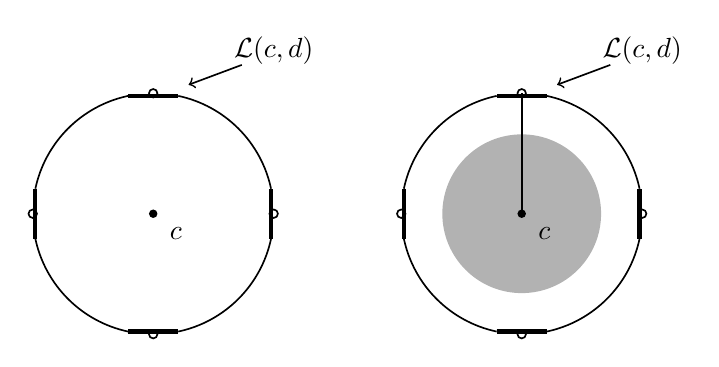
\begin{tikzpicture}[line width=0.6pt,scale=0.9]
  \def\cellshape{%
    \draw[line width=1.5pt] ({1.7*cos(78)},{1.7*sin(78)}) -- ({1.7*cos(102)},{1.7*sin(102)});
    \draw ({1.7*cos(102)},{1.7*sin(102)}) arc (102:168:1.7);
    \draw[line width=1.5pt] ({1.7*cos(168)},{1.7*sin(168)}) -- ({1.7*cos(192)},{1.7*sin(192)});
    \draw ({1.7*cos(192)},{1.7*sin(192)}) arc (192:258:1.7);
    \draw[line width=1.5pt] ({1.7*cos(258)},{1.7*sin(258)}) -- ({1.7*cos(282)},{1.7*sin(282)});
    \draw ({1.7*cos(282)},{1.7*sin(282)}) arc (282:348:1.7);
    \draw[line width=1.5pt] ({1.7*cos(348)},{1.7*sin(348)}) -- ({1.7*cos(12)},{1.7*sin(12)});
    \draw ({1.7*cos(12)},{1.7*sin(12)}) arc (12:78:1.7);
    \draw (0,1.7) circle (1.7pt);
    \draw (0,-1.7) circle (1.7pt);
    \draw (-1.7,0) circle (1.7pt);
    \draw (1.7,0) circle (1.7pt);
    \fill (0,0) circle (1.7pt);
  }
  \begin{scope}
    \cellshape
    \node at (0.32,-0.28) {$c$};
    \node at (1.7,2.3) {$\mathcal{L}(c,d)$};
    \draw[->] (1.25,2.1) -- (0.5,1.82);
  \end{scope}
  \begin{scope}[xshift=5.2cm]
    \fill[gray!60] (0,0) circle (1.12);
    \cellshape
    \draw (0,0) -- (0,1.7);
    \node at (0.32,-0.28) {$c$};
    \node at (1.7,2.3) {$\mathcal{L}(c,d)$};
    \draw[->] (1.25,2.1) -- (0.5,1.82);
  \end{scope}
\end{tikzpicture}
\caption{}
\label{fig:wbar-levels}
\end{figure}

\begin{proof}[\cref{thm:crossing-critical-value-homeomorphism}的证明]
由于 $\varGamma$ 的定义方式（见\cref{thm:sublevel-no-critical}的证明），我们知道：\trDiffeomorphism{} $\varGamma$ 把每一点都送到它自己那条\trTrajectory{}上的一个点。对 $(\lambda,x)\in\overline{W}^{\,u}(c,A+\varepsilon)$，如果经过 $x$ 的那条\trTrajectory{}并不终于 $d$（也就是说，如果 $x\notin W^s(d)$），那么我们便可以用 $\varGamma$ 来定义 $\chi(\lambda,x)$。因此，我们把我们的\trHomeomorphism{}定义在围绕
\[
P=\bigl\{(\lambda,x)\in\overline{W}^{\,u}(c,A+\varepsilon)\mid x\in W^s(d)\bigr\}
\]
的一个\trOpen{}集 $U$ 上，使得它能与\trHomeomorphism{} $\chi$ 良好地\trGluing——后者如\cref{thm:no-critical-interval-homeomorphism}中那样定义在 $U$ 的补集上。

\emph{我们先从 $\operatorname{Ind}(c)-\operatorname{Ind}(d)=1$ 且 $\operatorname{Ind}(d)\neq 0$ 的简单情形开始。}
在这种情形，
\[
P\subset\mathcal{M}(c,d)\subset W^u(c)\subset\overline{W}^{\,u}(c)\text{；}
\]
换言之，$P$ 只含有位于那些从 $c$ 到 $d$、高出水平 $A+\varepsilon$ 的\trTrajectory{}之上的点。在\trIndex{}之差的这个条件下，这些\trTrajectory{}所成之集 $\mathcal{L}(c,d)=\mathcal{M}(c,d)/\RR$ 是有限的。我们取定 $\ell\in\mathcal{L}(c,d)$，并设 $\tilde{\ell}\in\mathcal{M}(c,d)$ 为与之相对应的那条\trTrajectory（即把它看成 $V$ 中诸点所成之集）。设 $a$ 是这条\trTrajectory{}位于水平 $A+\varepsilon$ 处的点，即 $a=\tilde{\ell}\cap f^{-1}(A+\varepsilon)$；并设 $D\subset W^u(c)\cap f^{-1}(A+\varepsilon)$ 是一个维数为 $\operatorname{Ind}(d)$ 的小\trDisk，它在 $a$ 处与 $S_+(d)$ \trTransverse{}相交。\trSmale{}条件在这里起着本质性的作用。

\cref{thm:annulus-boundary}——它由\cref{fig:disk-descent}（那幅瓶状的图）所图示——告诉我们，把 $D-\{a\}$ 沿诸\trGradient{}线推入\trLevelSet{} $f^{-1}(A-\varepsilon)$ 时会发生什么。映射 $\varPhi$ 把它变成一个圆环 $C=S^{\operatorname{Ind}(d)-1}\times\,]0,\delta]$，后者与 $S_-(d)\cong S^{\operatorname{Ind}(d)-1}\times\{0\}$ 一起构成一个\trManifoldWithBoundary。我们回到这幅图（如今是\cref{fig:bottle-homeomorphism}）来描述我们的\trHomeomorphism{} $\chi$ 在 $\tilde{\ell}\cap\overline{W}^{\,u}(c,A+\varepsilon)$ 的邻域内的样子。

首先，$\chi$ 在 $\overline{W}^{\,u}(c,A+\varepsilon+\delta)$ 上是恒等。我们所考虑的
\[
\tilde{\ell}\cap\bigl(\overline{W}^{\,u}(c,A+\varepsilon)-\overline{W}^{\,u}(c,A+\varepsilon+\delta)\bigr)
\]
的邻域 $U$，是 $D$ 之上的一个圆柱（即瓶子的顶部），它由诸\trGradient{}线所定义，如\cref{fig:bottle-homeomorphism}中那样。图中还有第二个圆柱，记作 $\widetilde{U}$，含于 $f^{-1}([A-\varepsilon,A+\varepsilon])$ 之中：它就是瓶子的内部。它在顶部以 $D$ 为界，在底部以 $C\cup W^u(d,\varepsilon)$ 为界（而其侧面部分则由诸\trGradient{}线构成）。

我们选取一个\trHomeomorphism{} $\varGamma:U\to\widetilde{U}$，如\cref{fig:bottle-homeomorphism}中所描述的那样：\footnote{译注：原书此处印作 “as describe in Figure 4.11”；疑应为 “as described”（显见排印笔误）；中译文径按补全后文义译出。——译者注}
\begin{itemize}
\item $\varGamma$ 在 $U$ 的顶部部分上是恒等。
\item 在带阴影的部分上方，它就是\cref{thm:no-critical-interval-homeomorphism}中所定义的那个 $\varGamma$（特别地，在 $D-D'$ 上，它与\cref{thm:annulus-boundary}中所定义并使用的 $\varPhi$ 相重合）。
\item $\varGamma$ 把 $D'$ 送到 $W^u(d,\varepsilon)$ 上。
\end{itemize}

\begin{figure}[htbp]
\centering
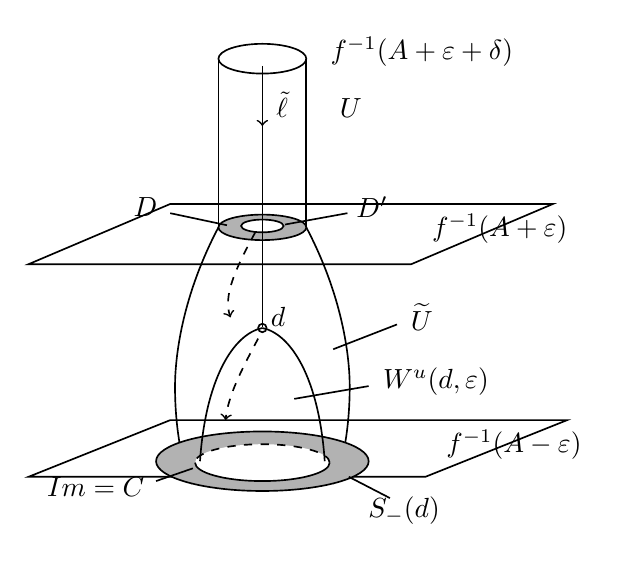
\begin{tikzpicture}[line width=0.6pt,scale=0.9]
  \draw (3.5,6.4) ellipse (0.62 and 0.21);
  \draw (2.88,6.40) -- (2.88,4.04);
  \draw (4.12,6.40) -- (4.12,4.04);
  \draw[->] (3.5,6.3) -- (3.5,5.45);
  \draw (3.5,5.45) -- (3.5,2.62);
  \node at (3.78,5.75) {$\tilde{\ell}$};
  \node at (4.75,5.7) {$U$};
  \node at (5.75,6.5) {$f^{-1}(A+\varepsilon+\delta)$};
  \draw (0.2,3.5) -- (2.2,4.35) -- (7.6,4.35) -- (5.6,3.5) -- cycle;
  \node at (6.85,4.0) {$f^{-1}(A+\varepsilon)$};
  \fill[gray!60] (3.5,4.02) ellipse (0.62 and 0.18);
  \fill[white] (3.5,4.04) ellipse (0.3 and 0.09);
  \draw (3.5,4.02) ellipse (0.62 and 0.18);
  \draw (3.5,4.04) ellipse (0.3 and 0.09);
  \draw (3.5,4.24) -- (3.5,3.82);
  \node at (1.85,4.3) {$D$};
  \draw (2.2,4.22) -- (3.0,4.05);
  \node at (5.05,4.3) {$D'$};
  \draw (4.7,4.22) -- (3.82,4.06);
  \draw (2.88,4.02) .. controls (2.50,3.30) and (2.30,2.55) .. (2.27,1.90)
        .. controls (2.25,1.30) and (2.36,0.62) .. (2.51,0.40);
  \draw (4.12,4.02) .. controls (4.50,3.30) and (4.70,2.55) .. (4.73,1.90)
        .. controls (4.75,1.30) and (4.64,0.62) .. (4.49,0.40);
  \draw (0.2,0.5) -- (2.2,1.3) -- (7.8,1.3) -- (5.8,0.5) -- cycle;
  \node at (7.05,0.95) {$f^{-1}(A-\varepsilon)$};
  \fill[gray!60] (3.5,0.72) ellipse (1.5 and 0.42);
  \fill[white] (3.5,0.7) ellipse (0.95 and 0.26);
  \draw (3.5,0.72) ellipse (1.5 and 0.42);
  \draw (2.55,0.7) arc (180:360:0.95 and 0.26);
  \draw[dashed] (4.45,0.7) arc (0:180:0.95 and 0.26);
  \node at (1.15,0.35) {$\operatorname{Im}\varPhi=C$};
  \draw (2.00,0.44) -- (2.52,0.62);
  \node at (5.5,0.02) {$S_-(d)$};
  \draw (5.30,0.20) -- (4.72,0.50);
  \draw (2.62,0.72) .. controls (2.70,1.90) and (3.10,2.52) .. (3.5,2.60);
  \draw (3.5,2.60) .. controls (3.90,2.52) and (4.30,1.90) .. (4.38,0.72);
  \draw (3.5,2.6) circle (1.7pt);
  \node at (3.72,2.75) {$d$};
  \draw[dashed,->] (3.4,3.95) .. controls (3.1,3.4) and (2.95,3.05) .. (3.05,2.75);
  \draw[dashed,->] (3.44,2.45) .. controls (3.2,2.0) and (3.02,1.65) .. (2.98,1.3);
  \node at (5.75,2.75) {$\widetilde{U}$};
  \draw (5.4,2.65) -- (4.5,2.3);
  \node at (5.95,1.85) {$W^u(d,\varepsilon)$};
  \draw (5.0,1.78) -- (3.95,1.6);
\end{tikzpicture}
\caption{}
\label{fig:bottle-homeomorphism}
\end{figure}

所要的\trHomeomorphism{}在 $U$ 上定义如下：
\[
\begin{cases}
\chi(x)=\varGamma(x) & \text{若 } x\notin D'\\
\chi(x)=(\ell,\varGamma(x)) & \text{若 } x\in D'\text{。}
\end{cases}
\]
在 $U$ 的侧面部分上，它与\cref{thm:no-critical-interval-homeomorphism}的那个\trHomeomorphism{}良好地\trGluing。由于 $\mathcal{L}(c,d)$ 是有限集，我们可以选取如上那种两两不交的诸邻域 $U$。于是，我们得到 $V$ 中有限多个（个数恰为 $n(c,d)$）圆柱 $U\cup\widetilde{U}$，它们只沿着 $W^u(d,\varepsilon)$ 相交。上面在这种圆柱之并上定义的映射 $\chi$，视作 $\overline{W}^{\,u}(c,A+\varepsilon)$ 中的映射时是\trInjective{}的；它还是连续的，这不难验证。当 $A$ 跨越\trCriticalValue{} $f(d)$ 时被添加到 $\overline{W}^{\,u}(c,A)$ 上去的那种集合 $\mathcal{L}(c,d)\times W^u(d,\varepsilon)$，确实包含在像之中；而在这些圆柱之外，$\chi$ 与\cref{thm:no-critical-interval-homeomorphism}所定义的映射良好地\trGluing。

我们可以不费力气地验证它是一个\trHomeomorphism，这就结束了这一情形的证明。

\emph{更一般的情形：$\operatorname{Ind}(c)-\operatorname{Ind}(d)$ 任意（且 $\operatorname{Ind}(d)\neq 0$）。}
我们需要在那些使 $x\in W^s(d)$ 的点 $(\lambda,x)\in\overline{W}^{\,u}(c,A+\varepsilon)$ 的邻域内定义 $\chi$：
\begin{enumerate}[label=(\alph*)]
\item 先像上一情形那样，考虑 $P$ 中位于 $\mathcal{M}(c,d)$ 内的那些点，也就是说，形如 $(\lambda,x)$ 而 $x\in W^u(c)\cap W^s(d)$ 的点\footnote{译注：原书本句印作“形如 $(\lambda,x)=x\in W^{u}(c)\cap W^{s}(d)$ 的点”；$(\lambda,x)$ 为点对，不能等于其第二分量，疑为排印衍文（多一枚等号），此处径删等号照文义译出。——译者注}。我们可以看出
\[
\mathcal{L}(c,d)=\mathcal{M}(c,d)\cap f^{-1}(A+\varepsilon)
\]
是 $W^u(c)\cap f^{-1}(A+\varepsilon)$ 的一个余维数为 $\operatorname{Ind}(d)$ 的\trSubmanifold。
设 $D$ 是 $\mathcal{L}(c,d)$ 在 $W^u(c)\cap f^{-1}(A+\varepsilon)$ 中的一个\trTubularNeighborhood：它是 $\mathcal{L}(c,d)$ 上一个维数为 $\operatorname{Ind}(d)$ 的\trDisk{}丛。对 $\ell\in\mathcal{L}(c,d)$，\trFiber{} $D_\ell$ 是一个\trDisk，它在 $a_\ell=\tilde{\ell}\cap f^{-1}(A+\varepsilon)$ 处与 $S_+(d)$ \trTransverse{}相交。于是，对每个 $\ell\in\mathcal{L}(c,d)$，我们都有一幅与\cref{fig:bottle-homeomorphism}相仿的图（把 $D$ 换成 $D_\ell$），以及一个以相仿方式定义的\trHomeomorphism{} $\varGamma_\ell:U_\ell\to U_\ell\cup\widetilde{U}_\ell$。诸圆柱 $\widetilde{U}_\ell$ 彼此只在 $W^u(d,\varepsilon)$ 上相交。然后，在位于 $D$ 之上、由诸\trGradient{}线所定义的那个圆柱丛 $U$ 上，我们如下定义 $\chi$：
\[
\begin{cases}
\chi(x)=\varGamma_\ell(x) & \text{若 } x\notin D'_\ell\\
\chi(x)=(\ell,\varGamma_\ell(x)) & \text{若 } x\in D'_\ell\text{，}
\end{cases}
\]
（当然，$D'_\ell$ 就是 $D'$ 的类似物）。
\item 现在考虑任意一点 $P$。它可以写成 $(\lambda,x)$，其中 $\lambda\in\overline{\mathcal{L}}(c,d')$、$x\in\mathcal{M}(d',d)$。请注意，当 $d'\neq c$ 时，这样的点 $x$ 并不在我们刚才于其上定义 $\chi$ 的那个定义域 $U$ 之中：事实上，$U$ 含于 $W^u(c)$ 之内。正如我们刚刚所证明的那样，我们可以在 $\mathcal{M}(d',d)\cap\{f\ge A+\varepsilon\}$ 的一个邻域 $U=U_{d'}$ 中定义 $\chi=\chi_{d'}$（这里 $d'$ 扮演 $c$ 的角色）。然后，我们在 $(\lambda,x)$ 于 $\overline{W}^{\,u}(c,A+\varepsilon)$ 中的邻域内如下定义 $\chi$：
\[
\chi(\lambda',y)=(\lambda',\chi_{d'}(y))\text{。}
\]
至此，我们已在 $P$ 的一个\trOpen{}邻域内定义了 $\chi$。请注意，$\chi$ 的像包含 $\overline{\mathcal{L}}(c,d)\times W^u(d,\varepsilon)$。我们像\cref{thm:no-critical-interval-homeomorphism}中那样把它延拓到整个 $\overline{W}^{\,u}(c,A+\varepsilon)$ 上，并毫不困难地验证它是一个\trHomeomorphism。
\end{enumerate}

\emph{为结束证明：$\operatorname{Ind}(d)=0$ 的情形。}
在这种情形，
\[
P=\bigl\{(\lambda,x)\in\overline{W}^{\,u}(c,A+\varepsilon)\mid x\in W^s(d)\bigr\}
\]
是 $\overline{W}^{\,u}(c,A+\varepsilon)$ 的一个\trConnectedComponent。
我们在 $P$ 上如下定义 $\chi$：
\[
\chi(\lambda,x)=
\begin{cases}
(\lambda,x) & \text{若 } f(x)\ge A+\varepsilon+\delta\\
(\lambda,\ell,d) & \text{若 } f(x)= A+\varepsilon\\
(\lambda,\varGamma(x)) & \text{若 } f(x)\in\,]A+\varepsilon,A+\varepsilon+\delta[\text{。}
\end{cases}
\]
（$\ell$ 表示 $x$ 的那条\trTrajectory。）在这个公式中，$\varGamma$ 是 $W^s(d)\cap f^{-1}\bigl(]A+\varepsilon,A+\varepsilon+\delta[\bigr)$ 与 $W^s(d)\cap f^{-1}\bigl(]f(d),A+\varepsilon+\delta[\bigr)$ 之间的一个\trDiffeomorphism，它由沿诸\trGradient{}线的推挤而得到。在其余的地方，我们用\cref{thm:no-critical-interval-homeomorphism}来定义 $\chi$，并（仍旧毫不费力地）验证它是一个\trHomeomorphism。

这个构造表明 $\chi$ 满足所要求的诸性质：它在 $\overline{W}^{\,u}(c,A+\varepsilon+\delta)$ 上的限制是恒等，并且 $\chi\bigl(W^u(c,A+\varepsilon)\bigr)=W^u(c,A-\varepsilon)$。这就结束了\cref{thm:crossing-critical-value-homeomorphism}的证明。
\end{proof}

以及\cref{thm:morse-cellular-isomorphism}的证明。
